% ==========================================
% BAB II STUDI LITERATUR
% ==========================================
\chapter{STUDI LITERATUR}
\label{chap:studi-literatur}

\section{Sistem Kelistrikan Gedung}
Sistem kelistrikan gedung merupakan rangkaian komponen dan instalasi yang berfungsi untuk menyalurkan energi listrik dari sumber ke berbagai beban di dalam bangunan secara aman, andal, dan efisien. Komponen utama yang mempengaruhi performa energi meliputi panel distribusi utama, panel distribusi per lantai atau subpanel, jaringan kabel dan penghantar, sistem proteksi, sistem pembumian, serta peralatan pemanfaat energi seperti sistem penerangan, sistem pemanas dan pendingin udara, motor listrik, dan peralatan khusus. Keberadaan sistem pengukuran menjadi elemen krusial, baik berupa meter energi utama maupun \textit{submetering} pada zona atau peralatan tertentu, karena kualitas dan granularitas data sangat mempengaruhi akurasi analisis \cite{hamdani2017audit}.

Kualitas daya listrik turut berpengaruh terhadap efisiensi konsumsi energi dan keandalan sistem. Ketidakseimbangan fasa dan faktor daya yang rendah dapat meningkatkan rugi-rugi energi, mempercepat degradasi peralatan, dan memicu gangguan operasional. Beban induktif seperti motor dan ballast serta beban nonlinier seperti inverter dan peralatan elektronik daya merupakan sumber utama permasalahan kualitas daya apabila tidak dikelola dengan baik. Studi lapangan yang memanfaatkan \textit{power meter} dan sistem pemantauan menunjukkan bahwa ketersediaan data primer memungkinkan identifikasi yang lebih akurat terhadap pemborosan energi dan anomali operasional sistem kelistrikan \cite{hamdani2017audit}.

Audit energi pada Gedung PPSDM Migas memperlihatkan bahwa sistem tata udara dan pencahayaan menjadi kontributor dominan konsumsi energi listrik, sehingga kedua subsistem tersebut menjadi fokus utama pengukuran dan analisis. Penelitian tersebut mendeskripsikan proses pengumpulan data lapangan yang mencakup pencatatan durasi operasi peralatan, pengukuran beban puncak, serta analisis pola penggunaan energi harian. Pola penggunaan energi ini digunakan untuk mengidentifikasi karakteristik konsumsi listrik dan peluang konservasi energi yang paling signifikan \cite{winarto2019audit}. Temuan ini mengindikasikan bahwa sistem kelistrikan gedung tidak hanya perlu dipahami dari sisi komponen fisik, tetapi juga dari sisi data operasional yang dihasilkan.

Selain karakteristik fisik dan operasional sistem kelistrikan, proses pengumpulan dan pencatatan data kelistrikan juga mempengaruhi kualitas evaluasi sistem. Implementasi audit energi berbasis antarmuka grafis menunjukkan bahwa penyajian data konsumsi dan parameter kelistrikan dalam format terstruktur dapat membantu auditor memahami kondisi sistem secara lebih konsisten dibandingkan pencatatan manual. Sistem audit IKE berbasis GUI yang dikembangkan menunjukkan bahwa representasi data yang sistematis mampu mereplikasi perhitungan manual dengan tingkat akurasi yang sama, serta mengurangi potensi kesalahan akibat penginputan data yang tidak konsisten \cite{fitri2022sistem}. Hal ini menegaskan bahwa karakteristik sistem kelistrikan gedung perlu dipahami tidak hanya dari sisi komponen dan beban, tetapi juga dari sisi bagaimana data operasionalnya dicatat, disimpan, dan dipresentasikan.

\section{Audit Energi pada Bangunan Gedung}
Audit energi pada bangunan gedung merupakan proses evaluasi sistematis terhadap penggunaan energi yang bertujuan untuk mendokumentasikan pola pemakaian energi, mengidentifikasi pemborosan, serta menyusun rekomendasi perbaikan yang terukur. Proses audit umumnya mencakup penentuan ruang lingkup, pengumpulan data historis dan data lapangan, pengukuran parameter energi, analisis pola beban listrik, perhitungan indikator kinerja energi, serta penyusunan laporan hasil audit. Hasil audit digunakan sebagai dasar pengambilan keputusan untuk intervensi teknis maupun perubahan operasional yang dapat meningkatkan efisiensi energi dan menurunkan biaya operasional \cite{putra2025evaluasi}.

Pelaksanaan audit energi dapat dibedakan berdasarkan tingkat kedalaman analisis, mulai dari audit cepat, audit awal, hingga audit investasi. Audit cepat berfokus pada identifikasi peluang penghematan yang mudah dan berbiaya rendah, sedangkan audit awal melibatkan pengukuran dan analisis yang lebih rinci untuk memperkirakan potensi penghematan. Audit investasi mencakup pengukuran mendalam, analisis teknis dan ekonomi, serta perencanaan implementasi yang didukung data primer. Perbedaan tingkat audit ini berimplikasi langsung pada kebutuhan data, kompleksitas perhitungan, dan tingkat dokumentasi yang diperlukan \cite{putra2025evaluasi}.

Agar hasil audit energi konsisten dan dapat dibandingkan, pelaksanaannya perlu mengacu pada pedoman dan standar yang berlaku. ISO 50001 menyediakan kerangka sistem manajemen energi yang mendorong organisasi untuk menetapkan kebijakan, sasaran, dan mekanisme perbaikan berkelanjutan. ISO 50002 memberikan panduan teknis mengenai metodologi audit energi, termasuk penentuan ruang lingkup, metode pengumpulan data, teknik pengukuran, serta struktur pelaporan. Pada tingkat nasional, SNI 03-6196-2000 mengatur prosedur audit energi pada bangunan gedung dan mendefinisikan indikator utama berupa intensitas konsumsi energi per satuan luas bangunan beserta klasifikasi tingkat efisiensinya \cite{iso2018_50001,iso2014_50002,sni2000_036196}.

Standar-standar tersebut pada dasarnya tersusun atas klausul dan persyaratan yang terstruktur, yang masing-masing mendefinisikan aspek proses audit, pengelolaan energi, metode pengukuran, serta format dokumentasi yang harus dipenuhi. Dalam praktik audit, pemenuhan klausul tersebut umumnya dievaluasi melalui peninjauan dokumen, observasi lapangan, dan verifikasi data pengukuran. Dengan demikian, kepatuhan terhadap standar tidak hanya berkaitan dengan penggunaan indikator yang tepat, tetapi juga dengan kelengkapan dokumentasi, konsistensi tahapan audit, serta keterlacakan proses evaluasi yang dilakukan. Struktur klausul ini secara konseptual memungkinkan proses audit dimodelkan dalam bentuk evaluasi terstruktur berbasis checklist terhadap setiap persyaratan yang relevan.

Kepatuhan terhadap standar umumnya diwujudkan melalui kesesuaian metode audit, indikator yang digunakan, serta struktur pelaporan hasil audit, meskipun tidak selalu dinyatakan dalam bentuk evaluasi kepatuhan formal. Studi audit energi berbasis pengukuran lapangan menunjukkan bahwa penerapan tahapan audit, pemilihan parameter energi, serta penggunaan indikator kinerja seperti intensitas konsumsi energi telah mengikuti kerangka audit energi yang direkomendasikan dalam standar, meskipun kepatuhan tersebut bersifat implisit \cite{hamdani2017audit,winarto2019audit}. Pendekatan ini menekankan bahwa kualitas audit lebih banyak ditentukan oleh konsistensi metode dan kejelasan dokumentasi dibandingkan dengan evaluasi kepatuhan berbasis checklist semata.

Pada penelitian yang mengintegrasikan perhitungan indikator kinerja secara lebih terstruktur, kepatuhan terhadap standar terlihat melalui penggunaan definisi indikator dan klasifikasi efisiensi yang mengacu pada pedoman nasional dan internasional. Sistem audit energi yang mengotomatisasi perhitungan intensitas konsumsi energi tetap mengandalkan rumus dan batas klasifikasi yang ditetapkan dalam standar, sehingga hasil yang diperoleh konsisten dengan praktik audit manual \cite{fitri2022sistem,putra2025evaluasi}. Hal ini menunjukkan bahwa peran utama standar dalam audit energi adalah sebagai acuan metodologis dan interpretatif, bukan sebagai mekanisme penilaian kepatuhan teknis yang kaku.

Dengan demikian, kepatuhan dalam audit energi bangunan gedung dapat dipandang sebagai kesesuaian proses audit, indikator, serta dokumentasi hasil terhadap struktur klausul dan pedoman yang berlaku. Perspektif ini menunjukkan bahwa kepatuhan tidak hanya merupakan keluaran naratif dalam laporan, tetapi dapat direpresentasikan sebagai entitas evaluatif yang terukur dan terdokumentasi. Oleh karena itu, terdapat peluang untuk mengembangkan perangkat lunak audit energi yang tidak hanya mengotomatisasi perhitungan indikator kinerja energi, tetapi juga membantu auditor memetakan dan menilai pemenuhan klausul standar secara sistematis.

Kepatuhan terhadap standar dan prosedur audit tidak hanya berdampak pada keseragaman metode, tetapi juga pada kualitas hasil audit yang dihasilkan. Studi empiris mengenai hubungan antara pemantauan, kepatuhan standar, dan mutu audit menunjukkan bahwa audit yang dilaksanakan dengan kerangka kerja yang jelas dan terdokumentasi menghasilkan temuan yang lebih andal serta mudah ditelusuri kembali. Kepatuhan terhadap standar meningkatkan konsistensi proses, mengurangi variasi penilaian antarauditor, dan memperkuat kepercayaan terhadap hasil audit \cite{owusuafriyiea2024monitoring}. Temuan ini menguatkan pentingnya penggunaan kerangka audit energi berbasis standar dalam praktik audit bangunan gedung.

Komponen sistem yang umumnya dianalisis dalam audit energi meliputi sistem penerangan, sistem pemanas dan pendingin udara, motor listrik, pompa, peralatan perkantoran, serta sistem pendukung seperti genset dan \textit{uninterruptible power supply}. Aspek pengukuran yang penting mencakup total konsumsi energi, beban puncak, pola beban listrik harian dan mingguan, serta faktor daya apabila relevan dengan permasalahan efisiensi. Penggunaan data primer dari meter energi dan \textit{submetering} memungkinkan analisis yang lebih akurat dibandingkan hanya mengandalkan data tagihan listrik \cite{hamdani2017audit}.

Hasil audit energi sering digunakan untuk menentukan prioritas tindakan penghematan. Pendekatan yang digunakan dapat berupa estimasi penghematan energi dan periode pengembalian modal, maupun metode pengambilan keputusan multikriteria untuk mengevaluasi alternatif intervensi berdasarkan kombinasi kriteria teknis, ekonomi, dan operasional \cite{putra2025evaluasi}. Oleh karena itu, perangkat lunak pendukung audit energi perlu dirancang untuk merepresentasikan alur kerja audit secara terstruktur, menyediakan modul akuisisi data, perhitungan indikator kinerja, mekanisme prioritisasi, serta penyajian laporan yang sesuai dengan format standar \cite{hermawan2022perencanaan}.

Pendekatan evaluasi berbasis klausul dan dokumentasi ini sejalan dengan konsep sistem pendukung audit yang menekankan pentingnya struktur, konsistensi, serta keterlacakan proses pengambilan keputusan \cite{dowling2007audit}. Dalam konteks audit energi, sistem yang dirancang untuk mendukung kepatuhan standar perlu mampu merepresentasikan tahapan audit, indikator yang dihitung, serta status pemenuhan setiap persyaratan sebagai bagian dari model data yang terintegrasi.

Selain itu, tingkat otomatisasi dalam sistem pendukung audit perlu dirancang secara seimbang. Otomatisasi perhitungan dan pelaporan dapat meningkatkan efisiensi dan konsistensi, namun auditor tetap memerlukan ruang untuk melakukan penilaian profesional terhadap kondisi lapangan yang spesifik. Konsep ini sejalan dengan kajian mengenai sistem pendukung audit yang menekankan pentingnya fleksibilitas dalam desain, sehingga sistem dapat berfungsi sebagai alat bantu keputusan tanpa menghilangkan peran auditor \cite{dowling2007audit}.

Audit energi juga dapat dipandang sebagai proses pengambilan keputusan yang terbantu oleh sistem. Kajian mengenai audit support systems menunjukkan bahwa sistem pendukung audit dapat dirancang dengan tingkat restriktivitas yang berbeda, mulai dari sistem yang hanya menyediakan checklist hingga sistem yang secara aktif mengarahkan alur audit dan menghasilkan rekomendasi otomatis. Sistem yang terstruktur dengan baik mampu meningkatkan efisiensi dan konsistensi audit, selama tetap memberikan ruang bagi auditor untuk melakukan penilaian profesional terhadap kondisi spesifik di lapangan \cite{dowling2007audit}. Perspektif ini relevan untuk audit energi gedung, di mana perangkat lunak berperan sebagai alat bantu keputusan yang mendukung, bukan menggantikan, peran auditor.

\section{Penilaian Kinerja Sistem Kelistrikan dalam Audit Energi}
Penilaian kinerja sistem kelistrikan dalam audit energi bertujuan untuk mengevaluasi tingkat efisiensi pemanfaatan energi listrik pada bangunan gedung berdasarkan indikator yang terukur dan dapat dibandingkan dengan nilai acuan. Penilaian kinerja tidak dimaksudkan untuk mengembangkan model matematis baru, melainkan untuk mengimplementasikan indikator kinerja yang telah direkomendasikan oleh standar dan praktik audit energi. Pendekatan ini memungkinkan hasil audit bersifat objektif, konsisten, dan dapat dipertanggungjawabkan \cite{iso2014_50002,sni2000_036196}.

Indikator kinerja utama yang digunakan dalam audit energi gedung adalah Intensitas Konsumsi Energi (IKE). IKE menyatakan besarnya konsumsi energi listrik tahunan yang dinormalisasi terhadap luas bangunan, sehingga memungkinkan perbandingan tingkat efisiensi antarbangunan atau antarperiode waktu. Secara matematis, nilai IKE dirumuskan seperti pada Persamaan~\ref{eq:ike}.

\begin{equation}
\mathrm{IKE} = \frac{E_{\text{tahunan}}}{A}
\label{eq:ike}
\end{equation}

Pada Persamaan~\ref{eq:ike}, $E_{\text{tahunan}}$ menyatakan total konsumsi energi listrik dalam satu tahun (kWh), sedangkan $A$ menyatakan luas bangunan (m$^2$). Nilai IKE umumnya dinyatakan dalam satuan kWh/m$^2$/tahun. Perhitungan IKE ini digunakan secara luas dalam audit energi gedung dan menjadi dasar klasifikasi tingkat efisiensi energi berdasarkan kategori yang telah ditetapkan dalam standar \cite{putra2025evaluasi,winarto2019audit}.

Hasil perhitungan IKE kemudian dibandingkan dengan nilai acuan atau batas klasifikasi efisiensi energi. Standar audit energi menyediakan kategori efisiensi seperti sangat efisien, efisien, cukup efisien, hingga boros, yang digunakan untuk menilai kinerja energi bangunan secara kualitatif berdasarkan nilai IKE yang diperoleh \cite{sni2000_036196}. Pendekatan klasifikasi ini memudahkan auditor dan pengelola gedung dalam menginterpretasikan hasil audit tanpa memerlukan analisis matematis yang kompleks.

Selain indikator utama berupa IKE, penilaian kinerja sistem kelistrikan juga dapat didukung oleh indikator pendamping yang bersifat deskriptif, seperti tren konsumsi energi antarperiode, distribusi beban antarzona, serta hasil pemeriksaan kepatuhan terhadap prosedur audit energi. Indikator-indikator tersebut tidak digabungkan ke dalam satu indeks matematis tunggal, melainkan disajikan secara terpisah sebagai dasar interpretasi dan rekomendasi perbaikan \cite{hamdani2017audit,fitri2022sistem}.

Rumus IKE dan mekanisme klasifikasi kinerja diimplementasikan secara langsung ke dalam sistem. Perangkat lunak berfungsi untuk mengotomatisasi perhitungan indikator, menyajikan hasil penilaian dalam bentuk visual dan laporan, serta mendukung keterlacakan proses audit. Dengan demikian, perangkat lunak tidak menggantikan prinsip audit energi yang ada, melainkan memperkuat konsistensi dan efisiensi penerapan penilaian kinerja sistem kelistrikan gedung \cite{iso2018_50001,iso2014_50002}.

\section{Rekayasa Perangkat Lunak untuk Penilaian Audit Energi}

Pengembangan perangkat lunak untuk penilaian audit energi memerlukan pendekatan yang terstruktur dan terdokumentasi dengan baik karena sistem yang dibangun harus mengacu pada standar audit energi yang jelas dan relatif stabil. Dalam rekayasa perangkat lunak, pendekatan pengembangan yang sistematis diperlukan untuk memastikan kebutuhan pengguna dan persyaratan domain dapat diterjemahkan secara konsisten ke dalam desain dan implementasi sistem \cite{sommerville2016software}. Perangkat lunak audit energi berperan sebagai sistem pendukung yang membantu auditor dalam mengelola data, melakukan perhitungan indikator kinerja energi, serta menyusun laporan hasil audit secara konsisten. Literatur menunjukkan bahwa sistem audit energi umumnya terdiri dari beberapa fungsi utama, yaitu akuisisi dan prapemrosesan data, perhitungan indikator kinerja, penentuan prioritas intervensi, serta visualisasi dan pelaporan hasil audit \cite{hermawan2022perencanaan}.

Fungsi akuisisi dan prapemrosesan data bertujuan untuk menerima data dari berbagai sumber, seperti data tagihan listrik, \textit{spreadsheet} hasil pencatatan lapangan, dan data pengukuran meter energi, kemudian melakukan normalisasi dan validasi sebelum data digunakan dalam proses analisis. Implementasi perangkat lunak audit energi berbasis antarmuka grafis menunjukkan bahwa otomasi proses input dan perhitungan dapat menghasilkan nilai indikator yang konsisten dengan perhitungan manual serta mengurangi beban kerja auditor dan potensi kesalahan \cite{fitri2022sistem}. Temuan ini menegaskan pentingnya tahap analisis kebutuhan yang jelas dalam pengembangan perangkat lunak audit energi, khususnya terkait format data dan aturan perhitungan yang digunakan \cite{sommerville2016software}.

Pada tahap desain dan implementasi sistem, integrasi data energi menjadi aspek penting karena data audit sering berasal dari berbagai sumber dengan struktur yang berbeda. Pendekatan ETL (\textit{extract, transform, load}) banyak digunakan untuk memastikan data yang masuk ke sistem telah melalui proses ekstraksi, transformasi, dan pemuatan yang terkontrol sehingga siap dianalisis secara akurat \cite{luciano2011integrating}. Prinsip ETL ini sejalan dengan pengembangan perangkat lunak berbasis Waterfall, di mana desain struktur data dan alur pemrosesan ditetapkan secara eksplisit sebelum tahap implementasi dilakukan \cite{sommerville2016software}.

Selain akurasi perhitungan, transparansi dan keterlacakan hasil audit merupakan kebutuhan penting dalam sistem audit energi. Konsep \textit{provenance} menekankan pentingnya dokumentasi asal data, tahapan pemrosesan, serta aturan atau logika yang digunakan dalam menghasilkan suatu hasil atau rekomendasi. Penerapan prinsip \textit{provenance} pada perangkat lunak audit energi mendukung proses pengujian dan evaluasi sistem, karena setiap hasil perhitungan dapat ditelusuri kembali ke data masukan dan aturan yang digunakan \cite{kale2023provenance}. Aspek ini relevan dalam tahap pengujian perangkat lunak untuk memverifikasi kesesuaian hasil dengan kebutuhan dan standar yang telah ditetapkan \cite{sommerville2016software}.

Kepatuhan terhadap standar dan prosedur audit juga berkaitan erat dengan kualitas keluaran sistem. Penelitian menunjukkan bahwa audit yang dilaksanakan dengan kerangka kerja yang selaras dengan standar menghasilkan proses dan hasil yang lebih konsisten serta dapat dipertanggungjawabkan \cite{owusuafriyiea2024monitoring}. Oleh karena itu, perangkat lunak audit energi perlu dirancang untuk mendukung tahapan audit dan format pelaporan sesuai ISO 50001, ISO 50002, dan SNI 03-6196-2000, sehingga sistem tidak hanya berfungsi sebagai alat komputasi, tetapi juga sebagai sarana dokumentasi audit yang terstandar.

Dengan demikian, rekayasa perangkat lunak untuk penilaian audit energi menuntut perancangan sistem yang terstruktur, terdokumentasi, dan berorientasi pada kebutuhan audit. Pendekatan pengembangan berbasis Waterfall memungkinkan setiap tahap, mulai dari analisis kebutuhan hingga pengujian, dilakukan secara sistematis dan dievaluasi terhadap persyaratan fungsional, akurasi perhitungan, serta kepatuhan terhadap standar audit energi \cite{sommerville2016software}. Literatur yang dibahas pada subbab ini menjadi dasar konseptual dalam merancang dan mengevaluasi perangkat lunak audit energi yang diusulkan pada penelitian ini.

\section{Penelitian Terdahulu}
Penelitian terdahulu digunakan sebagai dasar untuk memahami pendekatan, ruang lingkup, serta keterbatasan studi-studi yang berkaitan dengan audit energi dan pengembangan sistem pendukung audit. Ringkasan penelitian yang relevan disajikan pada Tabel~\ref{tbl:penelitianterdahulu}, yang memuat gambaran singkat mengenai fokus penelitian, kelebihan yang dihasilkan, serta keterbatasan masing-masing studi. Tinjauan ini menjadi landasan untuk mengidentifikasi celah penelitian dan merumuskan kontribusi pengembangan perangkat lunak audit energi yang diusulkan pada penelitian ini.

{
  \newlength{\LebarBersih}
  \setlength{\LebarBersih}{\dimexpr\textwidth-6\tabcolsep\relax}

  \newlength{\KolomDeskripsi}
  \newlength{\KolomIsi}

  \setlength{\KolomDeskripsi}{\dimexpr\LebarBersih/3\relax}
  \setlength{\KolomIsi}{\dimexpr\LebarBersih/3\relax}

  \newlength{\LebarTabel}
  \setlength{\LebarTabel}{%
    \dimexpr
      \KolomDeskripsi + 2\KolomIsi + 6\tabcolsep
    \relax
  }

  \newcommand{\JudulBlok}[4]{%
    \multicolumn{3}{@{}p{\LebarTabel}@{}}{%
      % \raggedright
      \vspace{-\dimexpr\baselineskip/2\relax}
      \hspace*{\tabcolsep}{%
        \hangindent=\tabcolsep
        \hangafter=1
        \rightskip=\tabcolsep
        #1\par
      }
      \vspace{-\dimexpr\baselineskip/2\relax}
      \rule{\LebarTabel}{0.4pt}\par
      % \vspace{-\dimexpr\baselineskip/8\relax}
      \begin{tabular}{%
        p{\KolomDeskripsi}%
        p{\KolomIsi}%
        p{\KolomIsi}}
        #2 & #3 & #4
      \end{tabular}
    }\\
  }

  \begin{longtable}{
    >{\raggedright\arraybackslash}p{\KolomDeskripsi}
    >{\raggedright\arraybackslash}p{\KolomIsi}
    >{\raggedright\arraybackslash}p{\KolomIsi}
  }
    \caption{Penelitian Terdahulu}\label{tbl:penelitianterdahulu}\\
    \toprule
    \textbf{Deskripsi} & \textbf{Kelebihan} & \textbf{Kekurangan} \\
    \midrule
    \endfirsthead

    \caption{Penelitian Terdahulu (lanjutan)} \\
    \toprule
    \textbf{Deskripsi} & \textbf{Kelebihan} & \textbf{Kekurangan} \\
    \midrule
    \endhead

    \midrule
    \multicolumn{3}{l}{\textit{Bersambung ke halaman berikutnya}}\\
    %\bottomrule
    \endfoot

    \bottomrule
    \endlastfoot

    % === Table Data ===
    \hline
    \JudulBlok{Audit Energi Sistem Kelistrikan Gedung Politeknik Negeri Ujung Pandang \cite{hamdani2017audit}}
    {Melakukan audit energi gedung dengan pengukuran parameter kelistrikan menggunakan \textit{power meter} dan sistem monitoring untuk menganalisis konsumsi energi dan kualitas data primer.}
    {Menghasilkan data pengukuran yang akurat dan mendukung identifikasi pemborosan energi secara detail.}
    {Proses audit dan analisis masih bersifat manual serta belum didukung oleh sistem perangkat lunak terintegrasi untuk pengolahan dan pelaporan.}
    \hline
    \hline
    \JudulBlok{Audit Energi Pada Gedung PPSDM Migas \cite{winarto2019audit}}
    {Menganalisis konsumsi energi gedung dengan fokus pada sistem tata udara dan pencahayaan melalui pencatatan durasi operasi, beban puncak, dan pola penggunaan energi.}
    {Memberikan gambaran praktis subsistem dominan konsumsi energi dan peluang konservasi yang signifikan.}
    {Belum menyediakan dukungan sistem informasi atau otomasi perhitungan dan dokumentasi audit.}
    \hline
    \hline
    \JudulBlok{Sistem Audit Intensitas Konsumsi Energi Listrik Berbasis GUI Matlab \cite{fitri2022sistem}}
    {Mengembangkan perangkat lunak berbasis antarmuka grafis untuk menghitung nilai IKE secara otomatis dari data konsumsi energi dan luas bangunan.}
    {Otomasi perhitungan IKE mengurangi kesalahan manual dan mempercepat proses evaluasi efisiensi energi.}
    {Cakupan sistem terbatas pada perhitungan IKE dan belum mendukung alur audit energi secara menyeluruh.}
    \hline
    \hline
    \JudulBlok{Evaluasi Intensitas Konsumsi Energi Melalui Audit Energi Listrik Gedung \cite{putra2025evaluasi}}
    {Menghitung IKE dan menggabungkannya dengan metode pengambilan keputusan multikriteria untuk menentukan prioritas strategi efisiensi energi.}
    {Menyediakan pendekatan terstruktur dalam penentuan prioritas intervensi berbasis data dan kriteria.}
    {Belum diimplementasikan dalam bentuk perangkat lunak audit energi yang terintegrasi.}
    \hline
    \hline
    \JudulBlok{Audit Support Systems and Decision Aids \cite{dowling2007audit}}
    {Mengkaji peran sistem pendukung audit dan tingkat restriktivitas sistem dalam mempengaruhi kualitas dan konsistensi proses audit.}
    {Memberikan kerangka konseptual desain sistem audit berbantuan perangkat lunak.}
    {Fokus pada audit laporan keuangan dan belum secara spesifik diterapkan pada audit energi bangunan.}
    \hline
  \end{longtable}
}

% Penelitian sebelumnya menunjukkan bahwa integrasi sistem monitoring permanen dan pengukuran primer meningkatkan kualitas audit energi serta mempermudah identifikasi tindakan konservasi energi \cite{hamdani2017audit}. Studi yang menggabungkan perhitungan indikator kinerja energi dengan metode pengambilan keputusan membantu menentukan prioritas intervensi berdasarkan ukuran dampak dan biaya \cite{putra2025evaluasi}. Penelitian tentang sistem informasi manajemen aset dan fasilitas menyoroti pentingnya model data yang baik dan alur kerja yang terstruktur untuk meningkatkan akurasi dan keterlacakan informasi \cite{hermawan2022perencanaan}. Studi tentang sistem pendukung audit dan bantuan keputusan mendeskripsikan kerangka desain sistem yang membatasi atau memberi kebebasan pada alur kerja auditor sehingga relevan untuk menentukan tingkat otomatisasi pada perangkat lunak audit energi \cite{dowling2007audit}.

% Audit energi pada Gedung PPSDM Migas menunjukkan bahwa sistem tata udara serta pencahayaan menjadi kontributor utama konsumsi energi sehingga pengukuran terfokus pada subsistem tersebut penting untuk identifikasi peluang penghematan \cite{winarto2019audit}. Sementara itu, implementasi perangkat lunak sederhana berbasis antarmuka grafis untuk perhitungan intensitas konsumsi energi dapat memperlihatkan bahwa otomasi perhitungan IKE mampu mereplikasi perhitungan manual dengan tingkat kesesuaian yang tinggi, sehingga mengurangi beban kerja manual dan potensi kesalahan \cite{fitri2022sistem}.

% Meskipun banyak studi memberikan bukti bahwa monitoring dan analisis terstruktur memberikan manfaat nyata, terdapat kebutuhan untuk perangkat lunak audit energi yang lebih terintegrasi dan dirancang untuk pengguna nonspesialis. Kesenjangan yang masih ada meliputi penggabungan akuisisi data dari berbagai sumber, engine perhitungan yang transparan, mekanisme scoring dan prioritisasi yang dapat dipahami oleh auditor, serta pembuatan laporan otomatis yang mudah digunakan. Kesenjangan inilah yang menjadi fokus pengembangan sistem dalam penelitian ini, yang akan diuji melalui studi kasus dan perbandingan hasil perangkat lunak dengan audit manual.


% \section{Penulisan Gambar, Tabel, Rumus, dan Kode}
% \lipsum[1]

% \subsection{Gambar}
% Contoh gambar dapat dilihat pada Gambar \ref{gambar:jaringan}. Gambar dan judulnya diposisikan di tengah. Nomor gambar tidak diakhiri tanda titik. Gambar tersebut dibuat menggunakan aplikasi draw.io dan disimpan ke format PNG setelah dengan zoom setting pada angka 300\%. Ukuran gambar yang ditampilkan dapat diatur dengan mengubah nilai \textit{width} dalam sintaks \textit{includegraphics}.

% \begin{figure}[t] % pilihan opsi yang disarankan: t = top, b = bottom, h = here
% 	\centering
%   \captionsetup{justification=centering}
%     	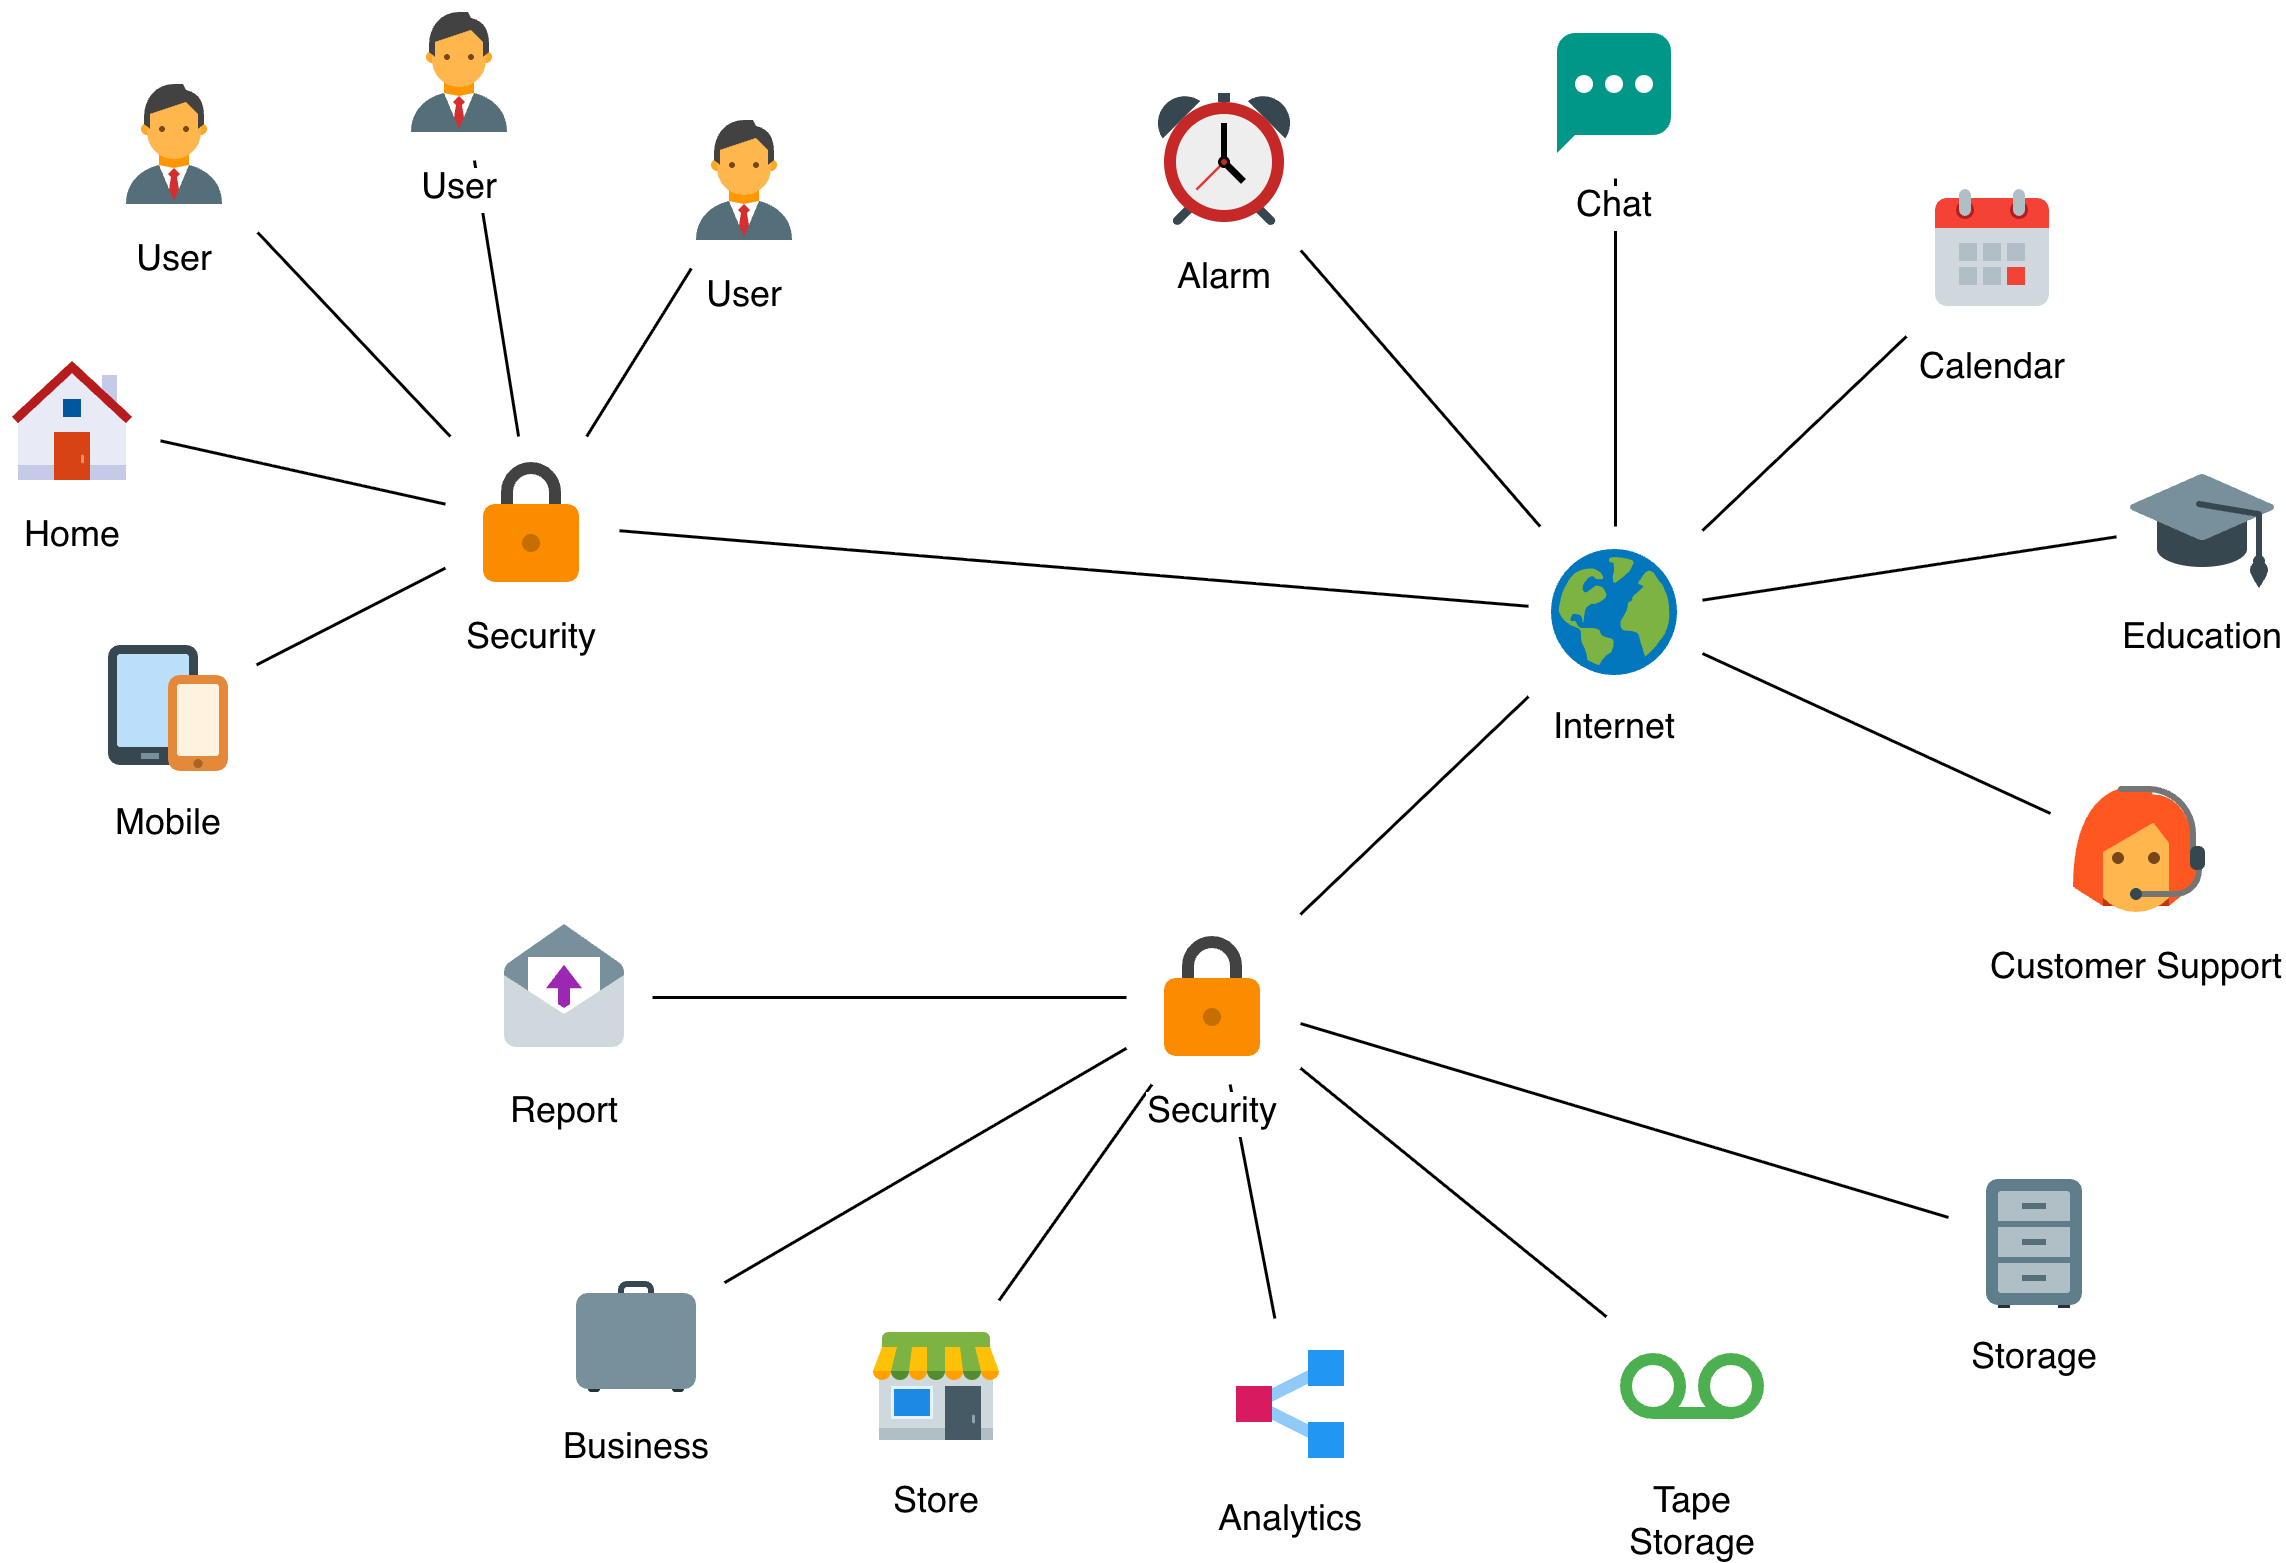
\includegraphics[width=0.7\textwidth]{image/gambar1.png}
% 	\caption{Contoh gambar jaringan}
% 	\label{gambar:jaringan}
% \end{figure}

% Gambar umumnya tidak jelas atau kabur jika gambar tersebut:
% \begin{enumerate}[a.]
%   \item diperoleh dari hasil cropping pada suatu halaman buku atau situs web;
%   \item hasil pembesaran gambar yang gambar aslinya sebenarnya berukuran kecil; atau
%   \item disimpan dalam resolusi kecil
% \end{enumerate}
% Ketidakjelasan gambar ini dapat dilihat pada garis-garis diagram yang tidak tegas dan tulisan-tulisan dalam gambar yang tampak kabur dan kurang jelas terbaca.

% Untuk mendapatkan gambar yang tidak kabur (\textit{blur}), langkah-langkah berikut dapat digunakan:
% \begin{enumerate}[(a)]
% \item Gambar yang didapat di suatu pustaka atau referensi sebaiknya digambar ulang, misalnya menggunakan PowerPoint, Canva, Figma, draw.io, atau yang lainnya.
% \item Jika diagram atau ilustrasi digambar menggunakan draw.io, saat gambar disimpan ke format PNG atau JPG (\textit{export as}), lakukan \textit{zoom} ke minimal 300\% (\textit{the default value is} 100\%). 
% \item Jika diagram digambar dengan menggunakan PowerPoint, gambar dapat langsung di-\textit{copy-paste} ke Word.
% \end{enumerate}

% \subsection{Tabel}
% Tabel ada dua jenis, yaitu tabel yang bisa termuat dalam satu halaman dan tabel yang sangat panjang sehingga tidak muat dalam satu halaman.
% \subsubsection{Tabel yang Muat dalam Satu Halaman}
% Contoh tabel dapat dilihat pada Tabel \ref{tbl:harga1} dan \ref{tbl:harga2}. Tabel dan judulnya dibuat rata kiri dan judul tabel diletakkan di atas tabel. Usahakan tabel dapat ditulis dalam satu halaman, tidak terpotong ke halaman berikutnya.

% \begin{table}[t] % pilihan opsi yang disarankan: t = top, b = bottom, h = here
%   \begin{tabular}{ | p{2cm} | p{2cm} | p{3cm} |}
% 	\hline
% 	Nama 	& Satuan 		& Harga \\
% 	\hline
% 	Buku 	& Exemplar	& 25000 \\
% 	Komputer	& Unit		& 2500000 \\
% 	Pensil	& Buah		& 118900 \\
% 	\hline
% 	\end{tabular}
% \caption{Tabel harga bahan pokok}
% \label{tbl:harga1}
% \end{table}



% \begin{table}[t] % pilihan opsi yang disarankan: t = top, b = bottom, h = here
% 	\begin{tabular}{ | l | c | r | }
% 	\hline
% 	Nama 	& Satuan 		& Harga \\
% 	\hline
% 	Buku 	& Exemplar	& 25000 \\
% 	Komputer	& Unit		& 2500000 \\
% 	Pensil	& Buah		& 118900 \\
% 	\hline
% 	\end{tabular}
% \caption{Tabel harga bahan sekunder}
% \label{tbl:harga2}
% \end{table}

% % -- Example of importing table from external file --
% \subsubsection{Mengimpor Tabel dari Berkas Eksternal}

% Tabel \ref{tbl:harga3} diimpor dari berkas eksternal \textit{table/tabel1.tex} menggunakan perintah \textit{input}. 
% Dengan demikian, jika tabel tersebut perlu diubah, cukup mengubah pada berkas eksternal tersebut tanpa perlu mengubah pada berkas utama ini.

% \input table/tabel1.tex


% % -- Example of long table --
% \subsubsection{Tabel yang Sangat Panjang}
% Jika tabel terlalu panjang sehingga tidak muat dalam satu halaman, gunakan paket 
% \textit{longtable} untuk membuat tabel yang dapat terpotong ke halaman berikutnya, 
% seperti pada Tabel \ref{tbl:longtable1}.

% \begin{longtable}{@{\extracolsep{\fill}} l c r r}
% \caption{Comprehensive Data Table Example}\label{tbl:longtable1} \\
% \toprule
% \textbf{ID} & \textbf{Name} & \textbf{Score} & \textbf{Rank} \\
% \midrule
% \endfirsthead

% \caption{Comprehensive Data Table Example (lanjutan)} \\
% \toprule
% \textbf{ID} & \textbf{Name} & \textbf{Score} & \textbf{Rank} \\
% \midrule
% \endhead

% \midrule
% \multicolumn{4}{r}{\textit{Bersambung ke halaman berikutnya}} \\
% %\bottomrule
% \endfoot

% \bottomrule
% \endlastfoot

% % === Table Data ===
% 1 & Alice Smith & 89 & 5 \\
% 2 & Bob Johnson & 93 & 3 \\
% 3 & Carol Davis & 95 & 2 \\
% 4 & Daniel Wilson & 88 & 6 \\
% 5 & Eve Thompson & 97 & 1 \\
% 6 & Frank Brown & 85 & 7 \\
% 7 & Grace Lee & 91 & 4 \\
% 8 & Henry Miller & 80 & 9 \\
% 9 & Irene Garcia & 83 & 8 \\
% 10 & Jack Robinson & 78 & 10 \\
% % Repeat with more rows to make it long
% 11 & Kevin Harris & 76 & 11 \\
% 12 & Laura Martin & 75 & 12 \\
% 13 & Michael Clark & 74 & 13 \\
% 14 & Natalie Lewis & 73 & 14 \\
% 15 & Olivia Walker & 72 & 15 \\
% 16 & Peter Hall & 71 & 16 \\
% 17 & Quinn Allen & 70 & 17 \\
% 18 & Rachel Young & 69 & 18 \\
% 19 & Samuel King & 68 & 19 \\
% 20 & Tina Wright & 67 & 20 \\
% 21 & Uma Scott & 66 & 21 \\
% 22 & Victor Green & 65 & 22 \\
% 23 & Wendy Adams & 64 & 23 \\
% 24 & Xavier Nelson & 63 & 24 \\
% 25 & Yolanda Carter & 62 & 25 \\
% 26 & Zachary Perez & 61 & 26 \\
% 27 & Amelia Baker & 60 & 27 \\
% 28 & Benjamin Rivera & 59 & 28 \\
% 29 & Charlotte Rogers & 58 & 29 \\
% 30 & David Murphy & 57 & 30 \\
% 31 & Ethan Cooper & 56 & 31 \\
% 32 & Fiona Reed & 55 & 32 \\
% 33 & George Bailey & 54 & 33 \\
% 34 & Hannah Cox & 53 & 34 \\
% 35 & Isaac Howard & 52 & 35 \\
% 36 & Julia Ward & 51 & 36 \\
% 37 & Kyle Flores & 50 & 37 \\
% 38 & Lily Bell & 49 & 38 \\
% 39 & Mason Sanders & 48 & 39 \\
% 40 & Nora Patterson & 47 & 40 \\
% 41 & Owen Ramirez & 46 & 41 \\
% 42 & Penelope Torres & 45 & 42 \\
% 43 & Quentin Foster & 44 & 43 \\
% 44 & Rebecca Gonzales & 43 & 44 \\
% 45 & Sebastian Bryant & 42 & 45 \\
% 46 & Taylor Alexander & 41 & 46 \\
% 47 & Ursula Russell & 40 & 47 \\
% 48 & Vincent Griffin & 39 & 48 \\
% 49 & William Diaz & 38 & 49 \\
% 50 & Zoe Simmons & 37 & 50 \\
% % (You can easily extend this list to hundreds of rows)
% \end{longtable}

% \subsubsection{Beberapa Contoh Penulisan Rumus atau Persamaan Matematika Menggunakan LaTeX Termasuk Penomorannya}
% Contoh rumus matematika dapat ditulis seperti pada Persamaan \ref{eq:contoh1} di bawah ini. 
% Penomoran persamaan diletakkan di sebelah kanan, dan rumus ditulis dalam mode \textit{display math}.
% \begin{equation}
% E = mc^2
% \label{eq:contoh1}
% \end{equation}

% Contoh lain penulisan rumus matematika yang lebih kompleks dapat ditulis seperti pada Persamaan \ref{eq:rumus2}.

% \begin{align}
% f(x) &= ax^2 + bx + c \\
% f'(x) &= \frac{d}{dx}(ax^2 + bx + c) \notag \\ % tidak menampilkan nomor pada baris ini
%       &= 2ax + b \label{eq:rumus2}
% \end{align}

% Jika rumus terlalu panjang untuk ditulis dalam satu baris, gunakan lingkungan \textit{multline} seperti pada Persamaan \ref{eq:rumus3} di bawah ini.
% \begin{multline} 
% y = a_0 + a_1x + a_2x^2 + a_3x^3 + a_4x^4 + a_5x^5 + a_6x^6 + a_7x^7 \\
%     + a_8x^8 + a_9x^9 + a_{10}x^{10} \label{eq:rumus3}
% \end{multline}

% Jika ada penurunan rumus yang terdiri dari beberapa baris, namun tidak memerlukan penomoran pada setiap baris, gunakan lingkungan \textit{align*}, misalnya:

% \begin{align*} 
% S &= \sum_{i=1}^{n} i^2 \\
%   &= 1^2 + 2^2 + 3^2 + \cdots + n^2 \\
%   &= \frac{n(n + 1)(2n + 1)}{6}
% \intertext{Contoh lainnya adalah rumus untuk mencari nilai rata-rata fungsi $f(x)$ pada interval $[p, q]$:}
% \bar{f} &= \frac{1}{q - p} \int_{p}^{q} f(x) \, dx \\
%         &= \frac{1}{q - p} \int_{p}^{q} (ax^2 + bx + c) \, dx \\
%         &= \frac{1}{q - p} \left[ \frac{a}{3}x^3 + \frac{b}{2}x^2 + cx \right]_p^q \\
%         &= \frac{a(q^3 - p^3)}{3(q - p)} + \frac{b(q^2 - p^2)}{2(q - p)} + c \label{eq:rumus4}
% \end{align*}



% \subsection{Algoritma, Pseudocode, atau Kode}
% Contoh penulisan algoritma atau pseudocode dapat ditulis seperti pada Kode \ref{alg:contoh1} di bawah ini. 
% Gunakan paket \textit{listings} untuk menulis source code dalam bahasa pemrograman tertentu, seperti pada Kode \ref{lst:contoh1}. 


% % -- Example of pseudocode and source code listing --
% % -- Gunakan minipage agar listing tidak terpotong ke halaman berikutnya --
% \begin{minipage}{\textwidth} 
% \begin{lstlisting}[frame=lines, captionpos=t, caption={Contoh pseudocode}, label={alg:contoh1}]
% ALGORITHM HelloWorld
%    PRINT "Hello, World!"
% END ALGORITHM
% \end{lstlisting}
% \end{minipage}

% \begin{minipage}{\textwidth}
% \begin{lstlisting}[language=Python, frame=single, caption={Contoh source code Python}, captionpos=t, label={lst:contoh1}]
% def hello_world():
%     print("Hello, World!")       
% hello_world()
% \end{lstlisting}
% \end{minipage}


% \section{Beberapa Kesalahan Penulisan yang Sering Terjadi}
% \subsection{Penggunaan Kata "di mana" atau "dimana"}
% Banyak yang menuliskan kata "di mana" atau "dimana" sebagai pengganti kata "which" dalam bahasa Inggris. 
% Padahal, penggunaan kata "di mana" atau "dimana" tidak tepat dalam konteks tersebut. Demikian juga untuk kata serupa, misalnya "yang mana".
% Kata "di mana" atau "dimana" ini harus diganti dengan kata lain, seperti "dengan", "tempat", "yang", dan sebagainya tergantung kalimatnya.
% Penjelasan lengkap dapat dilihat pada \autocite{BPBI}.

% \subsection{Penggunaan Kata "sedangkan" dan "sehingga"}

% \begin{table}[t]
%   \begin{tabular}{|c|l|l|}
%   \hline
%   Kata & Salah & Benar \\ \hline
%   sedangkan & \begin{tabular}[c]{@{}c@{}}Sedangkan sistem lama masih\\ digunakan oleh banyak pengguna.\end{tabular} & \begin{tabular}[c]{@{}c@{}}Sistem lama masih digunakan\\ oleh banyak pengguna,\\ sedangkan sistem baru belum siap.\end{tabular} \\ \hline
%   sehingga & \begin{tabular}[c]{@{}c@{}}Sehingga sistem lama masih\\ digunakan oleh banyak pengguna.\end{tabular} & \begin{tabular}[c]{@{}c@{}}Sistem lama masih digunakan\\ oleh banyak pengguna sehingga\\ sistem baru belum siap.\end{tabular} \\ \hline
%   \end{tabular}
%   \caption{Contoh penggunaan kata "sedangkan" dan "sehingga"}
%   \label{tbl:sedangkan_sehingga}
% \end{table}

% Kata "sedangkan" dan "sehingga" adalah kata hubung atau konjungsi. 
% Konjungsi adalah kata atau ungkapan yang menghubungkan satuan bahasa 
% (kata, frasa, klausa, dan kalimat). 
% Konjungsi dapat dibagi menjadi konjungsi intrakalimat dan antarkalimat.  
% Kata "sedangkan" menghubungkan dua klausa yang bersifat kontrasif, 
% sedangkan "sehingga" menghubungkan dua klausa yang bersifat kausal. 
% Dalam ragam formal, kata hubung “sedangkan” dan “sehingga” hanya dapat digunakan 
% sebagai konjungsi intrakalimat sehingga kedua konjungsi itu \textbf{tidak dapat diletakkan pada awal kalimat}.
% Selain itu, penggunaan kata "sedangkan" harus didahului oleh koma (,), sedangkan kata "sehingga" tidak perlu didahului oleh koma (,).
% Contoh penggunaan yang benar dan salah dapat dilihat pada Tabel \ref{tbl:sedangkan_sehingga}.


% \subsection{Penggunaan Istilah yang Tidak Baku}
% Ada beberapa istilah yang sering digunakan dalam pembicaraan sehari-hari, tetapi tidak baku dalam penulisan ilmiah.
% Beberapa istilah tersebut antara lain:
% \begin{enumerate}
%   \item analisa $\rightarrow$ analisis
%   \item eksisting atau existing $\rightarrow$ yang ada atau saat ini
%   \item bisnis proses $\rightarrow$ proses bisnis
%   \item user $\rightarrow$ pengguna
%   \item system $\rightarrow$ sistem
%   \item database $\rightarrow$ basis data
%   \item aktifitas $\rightarrow$ aktivitas
%   \item efektifitas $\rightarrow$ efektivitas
%   \item sosial media $\rightarrow$ media sosial
% \end{enumerate}

% \subsection{Pemisah Desimal dan Ribuan}
% Tanda pemisah desimal dalam bahasa Indonesia adalah tanda koma, contoh:
% \begin{enumerate}
%   \item (Salah) Akurasi naik menjadi 50.6\% 
%   \item (Benar) Akurasi naik menjadi 50,6\% 
% \end{enumerate}

% \subsection{Daftar atau \textit{List}}
% Ada beberapa aturan penulisan daftar atau \textit{list} yang perlu diperhatikan, antara lain:
% \begin{enumerate}[a)]
% \item Jika memungkinkan, hindari penggunaan “bullet points” atau sejenisnya. Sebaiknya, gunakan angka (1, 2, 3, ...) atau huruf (a, b, c, …). Dengan demikian, pembaca dapat dengan mudah melihat jumlah \textit{item} atau \textit{list}. 
% \item Jika dalam daftar hanya ada satu item, tidak perlu menggunakan nomor urut.
% \item Penjelasan atau deskripsi suatu item sebaiknya menyatu dengan judul item tersebut, tidak berbeda halaman. Contoh yang salah: judul item ada di halaman 10, namun deskripsinya di halaman 11. Sebaiknya pindahkan judul tersebut ke halaman 11.
% \item Jika penjelasan atau deskripsi suatu item cukup panjang, misalnya lebih dari 1 halaman atau terdiri atas beberapa paragraf, sebaiknya setiap item tersebut dijadikan judul subbab, kecuali jika level subbab sudah mencapai level 4. 
% \end{enumerate}

% \subsection{Penggunaan Kata "masing-masing" dan "setiap"}
% Kata “masing-masing” digunakan di belakang kata yang diterangkan, misalnya 
% "Setiap proses menggunakan algoritma masing-masing". Kata “tiap-tiap” atau “setiap”
% ditempatkan di depan kata yang diterangkan, misalnya
% "Setiap proses menggunakan algoritma tertentu".
